% -*- compile-command: "cd .. && make -k tex/case-study-research-ide.pdf" -*-
\documentclass[document.tex]{subfiles}
\begin{document}
\chapter{Case~Study: An~IDE~for~Research}
\label {ch:case-study-2}

While the first case study focused on a system with several complex, deadline-driven workflows, it had only a simple notion of roles. The second case study balances this by focusing on an application that has a simple and well-known workflow, but a more complex notion of user roles.

\sectionnote {AC}
\section {Background}
\label{sec:case-study-research-background}

Workflow-based systems have found a niche in computational science and bioinformatics. Software suites called scientific workflow systems allow researchers to describe their experiments in terms of workflows and manage the results that they produce. These tools improve reproducibility by allowing scientists to share the steps required to reproduce an experiment, and review how the experiment's results were produced.

Taverna is one such scientific workflow system \cite{taverna-website}. It is an open source tool build to aid in the execution of scientific experiments, with a focus on in silico experiments. In silico experiments are scientific experiments which are done entirely on a computer such as complex models of cells. The main benefit to in silico experiments is the increased precision and the size of the data that can be generated and analyzed. Unfortunately, many researchers are not programmers and are unable to easily create in silico experiments. Taverna allows a researcher to describe an experiment with a workflow so that the steps of an experiment are abstracted from the programming of it. This modular workflow approach allows a researcher to design an experiment without having to worry about the technical details of programming.

Due to the large computational requirement of in silico experiments Taverna allows multiple systems to work on the computations of a single experiment. This allows a researcher to utilize an entire network of computers and benefit from the extra computational power. Because of the nature many scientific experiments many tasks are able to be done in parallel. With parallel activities and enough computational power the speed at which an experiment can be completed drastically increases.


\sectionnote {BM}
\section {Overview}
\label{sec:case-study-research-overview}

Scientific misconduct and issues with reproducibility are a growing concern.
While scientific workflow tools similar to Taverna have data management features that help researchers to track data provenance and reproducibility, they do not make any attempt to manage the scientific process itself. Though deliberate misconduct and fraud are difficult to prevent using technological means, it should be possible to encourage best practices by using a software tool to guide inexperienced researchers through the scientific process, which can itself be modeled as a workflow.

In general, the process of performing a research project can be described in six steps:
\begin{compactenum}
\item \textbf{Write a hypothesis}
\item \textbf{Perform a literature review} to discover prior work in the field, summarize the context of the work, and perhaps gain ideas for design of the experiment.
\item \textbf{Design an experimental method} to test the hypothesis.
\item \textbf{Record the results} obtained from the experiment.
\item \textbf{Analyze the results}, often using a set of domain-specific tools.
\item \textbf{Draw conclusions} from the analysis.
\end{compactenum}

Though the process is often taught as a sequence of steps, some iteration may occur occasionally; for example, while designing the method a researcher might realize that their hypothesis as written is unclear or difficult, and alter it to correct the issue. On the other hand, there are several patterns of changes that should not be made, in order to avoid introducing biases or outright fraud:
\begin{compactitem}
\item the hypothesis and method should not be edited after the experiment begins;
\item the results should not be changed after beginning analysis;
\item the analysis, conclusions, and literature review should always be editable.
\end{compactitem}

The research process itself may be carried out by a number of individuals with different responsibilities, depending on the discipline. For example, a technician may be responsible for validating the methodology and carrying out the experiment itself, while a statistician may be consulted for the analysis. It is important that a tool for managing the research process can accommodate any arbitrary assignment of responsibilities to individuals that a project demands.

As a well-defined sequence of steps with restricted iteration, this process seems like an excellent candidate for automation using a workflow framework. Furthermore, as user roles are not predefined, but instead specified on a project-by-project basis, this case study provides an opportunity to investigate best practices and existing libraries for role-based access.
It also fills a different need that isn't met by existing existing scientific workflow software. \todo{Something about synergy.}


\sectionnote {AC}
\section {Requirements}
\label{sec:case-research-requirements}

  Figures \ref{fig:case-research-use-case-project-management} through \ref{fig:case-research-use-case-project-workflow} display the individual use cases for the research IDE application. They have been separated into two diagrams based on project management and the main project workflow. The project management shown in Figure \ref{fig:case-research-use-case-project-management} goes over which actors have permission to view, create and delete research projects. In addition, it also displays modifying the permissions of users for a given project and how the project advances to the next stage of the workflow. The project workflow shown in Figure \ref{fig:case-research-use-case-project-workflow} focuses on the workflow system described in section \ref{sec:case-study-research-overview}.

\begin{figure}[!ht]
\centering 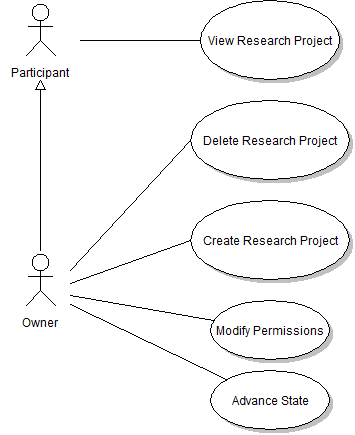
\includegraphics[height=5in]{./img/case-study-research-railgun/project_management_use_case}
\caption{Use case diagram for the project management functionality of the research IDE.}
\label{fig:case-research-use-case-project-management}
\end{figure}

\begin{figure}[!ht]
\centering 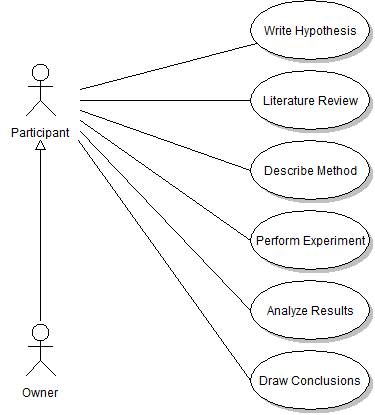
\includegraphics[height=5in]{./img/case-study-research-railgun/project_workflow_use_case}
\caption{Use case diagram for the project workflow functionality of the research IDE.}
\label{fig:case-research-use-case-project-workflow}
\end{figure}

\FloatBarrier

  The two actors Owner and Participant represent the two roles in the research IDE. Owners own projects and participants participate in projects. Any user is able to create a project which then assigns their role as the owner of that project. As an owner of a project the user has all permissions granted to them and is able to grant permissions to participants for specific stages of the workflow. There are two permission types: view, and edit. The view permission allows access to view specific stages of a workflow and the edit permission allows a participant to make modifications to the project in that stage of the workflow.

  Tables \ref{tbl:use-case-view-research-project} to \ref{tbl:use-case-advance-state} display the use case descriptions for the project management diagram shown above. Tables \ref{tbl:use-case-write-hypothesis} to \ref{tbl:use-case-draw-conclusions} display the use case descriptions for the above project workflow diagram. These descriptions describe exactly what permissions are required to do actions during each use case.
 
\begin{table}
  \centering
  \caption{Use case description for the ``View Research Project'' use case of the research IDE system.}
  \label{tbl:use-case-view-research-project}

  \begin{usecase}[View Research Project]
    \ucpart{Description}
    A User can view information about a project that he has permissions with.
    %
    \ucpart{Actors}
    Owner, Participant
    %
    \ucpart{Preconditions}
    The Research Project Exists and the User accessing it has at least one permission to view a task in the project.
    %
    \ucpart{Flow}
    \ucnormal
    \begin{ucenum}
      \item The User selects a research project from a list of projects that the User has access to.
      \item The User is shown detailed information about the project: current state of project, and any sections the user is allowed to view/edit.
    \end{ucenum}
    %
    \ucpart{Exceptions}
    \ucexception{No Permissions}
    The User has no permissions to view the project and is redirected back to a list of projects he has permission to view and an error is shown.
    %
    \ucpart{Postconditions}
    The User is brought to a details view of the selected project.
  \end{usecase}
\end{table}


\begin{table}
  \centering
  \caption{Use case description for the ``Delete Research Project'' use case of the research IDE system.}
  \label{tbl:use-case-delete-research-project}

  \begin{usecase}[Delete Research Project]
    \ucpart{Description}
    A Research Project can be deleted by the Owner of that project at any time.
    %
    \ucpart{Actors}
    Owner
    %
    \ucpart{Preconditions}
    The Research Project to be deleted exists.
    %
    \ucpart{Flow}
    \ucnormal
    \begin{ucenum}
      \item The User selects to delete the project.
      \item A confirmation box appears and the User agrees.
      \item The Project is deleted and the User is sent to a list of projects he has permission to view.
    \end{ucenum}
    %
    \ucpart{Variations}
    \ucbranch{A}
    \begin{ucenum}
      \item [A.2] A confirmation box appears and the User disagrees.
      \item [A.3] The User returns the the details view of that project.
    \end{ucenum}
    %
    \ucpart{Exceptions}
    \ucexception{Not Owner}
    A participant cannot delete a project he does not own. He is redirected back to the list of projects he has permission to view.
    %
    \ucpart{Postconditions}
    The Research Project is deleted from the system.
  \end{usecase}
\end{table}


\begin{table}
  \centering
  \caption{Use case description for the ``Create Research Project'' use case of the research IDE system.}
  \label{tbl:use-case-create-research-project}

  \begin{usecase}[Create Research Project]
    \ucpart{Description}
    A Research Project can be created by any User and that User becomes the Owner of that project.
    %
    \ucpart{Actors}
    Owner
    %
    \ucpart{Flow}
    \ucnormal
    \begin{ucenum}
      \item The User selects to Create a new Research Project.
      \item The User submits a name and description for the project.
      \item The Research project is created, The User is assigned as the owner and is redirected to viewing the project.
    \end{ucenum}
    %
    \ucpart{Postconditions}
    The Research Project is created and the User is assigned to the Owner of the project.
  \end{usecase}
\end{table}


\begin{table}
  \centering
  \caption{Use case description for the ``Modify Permissions'' use case of the research IDE system.}
  \label{tbl:use-case-modify-permissions}

  \begin{usecase}[Modify Permissions]
    \ucpart{Description}
    The Owner of a project can modify the permissions of other Users for his project.
    %
    \ucpart{Actors}
    Owner
    %
    \ucpart{Preconditions}
    The User is the Owner of the project to which he is assigned permissions.
    %
    \ucpart{Flow}
    \ucnormal
    \begin{ucenum}
      \item The User selects to modify the permissions for his project.
      \item A list of other Users on the system is shown along with their current.
      \item The User selects a specific permission to modify and submits the change.
      \item The other User now has the selected permissions for the project.
    \end{ucenum}
    %
    \ucpart{Exceptions}
    \ucexception{Cannot Modify Owner Permissions}
    The Owner always has every permission and this cannot be changed, redirected back to project view.
    \ucexception{Not Owner}
    Only Owners can modify permissions, redirected back to project view.
    %
    \ucpart{Postconditions}
    The User who had his permissions modified can now do any actions that require that permission.
  \end{usecase}
\end{table}


\begin{table}
  \centering
  \caption{Use case description for the ``Advance State'' use case of the research IDE system.}
  \label{tbl:use-case-advance-state}

  \begin{usecase}[Advance State]
    \ucpart{Description}
    The Owner can advance the state of the project as long as something has been saved into the current state.
    %
    \ucpart{Actors}
    Owner
    %
    \ucpart{Preconditions}
    There is another state in the workflow after the current state.
    %
    \ucpart{Flow}
    \ucnormal
    \begin{ucenum}
      \item The User selects to advance the state of the project
      \item There is something saved for the current state and the state is advanced to the next state in the workflow.
    \end{ucenum}
    %
    \ucpart{Variations}
    \ucbranch{A}
    \begin{ucenum}
      \item [A.2] There is nothing saved for the current state and a message is shown notifying the User that something must be saved before moving on.
    \end{ucenum}
    %
    \ucpart{Exceptions}
    \ucexception{Not Owner}
    A participant cannot advance the state of a project. He is redirected back to the project view
    \ucexception{Last State}
    There is no state after the current state so the state cannot be advanced, User is redirected back to project view.
    %
    \ucpart{Postconditions}
    The state of the workflow is advanced to the next state.
  \end{usecase}
\end{table}


\begin{table}
  \centering
  \caption{Use case description for the ``Write Hypothesis'' use case of the research IDE system.}
  \label{tbl:use-case-write-hypothesis}

  \begin{usecase}[Write Hypothesis]
    \ucpart{Description}
    A User with the correct permissions can edit or view the hypothesis of the current project.
    %
    \ucpart{Actors}
    Owner, Participant
    %
    \ucpart{Preconditions}
    The workflow must be in the ‘Write Hypothesis”, “Literature Review” or “Describe Method” state. The User has the ‘edit’ or ‘view’ permission for this task.
    %
    \ucpart{Flow}
    \ucnormal
    \begin{ucenum}
      \item The User selects to write the hypothesis.
      \item The User has the ‘edit’ permission and makes a modification to the hypothesis and selects to save.
      \item The Hypothesis is updated and saved.
    \end{ucenum}
    %
    \ucpart{Variations}
    \ucbranch{A}
    \begin{ucenum}
      \item [A.2] The User has the ‘view’ permission and does not have the ‘edit’ permission and is shown the current hypothesis.
    \end{ucenum}
    %
    \ucpart{Exceptions}
    \ucexception{No Permission}
    The User does not have permission to ‘edit’ or ‘view’ the hypothesis and is returned to project view.
  \end{usecase}
\end{table}


\begin{table}
  \centering
  \caption{Use case description for the ``Literature Review'' use case of the research IDE system.}
  \label{tbl:use-case-literature-review}

  \begin{usecase}[Literature Review]
    \ucpart{Description}
    A User with the correct permissions can edit or view the literature review of the current project.
    %
    \ucpart{Actors}
    Owner, Participant
    %
    \ucpart{Preconditions}
    The workflow must be in the “Literature Review” or “Describe Method” state. The User has the ‘edit’ or ‘view’ permission for this task.
    %
    \ucpart{Flow}
    \ucnormal
    \begin{ucenum}
      \item The User selects to work on the literature review.
      \item The User has the ‘edit’ permission and makes a modification to the literature review and selects to save.
      \item The Literature Review is updated and saved.
    \end{ucenum}
    %
    \ucpart{Variations}
    \ucbranch{A}
    \begin{ucenum}
      \item [A.2] The User has the ‘view’ permission and does not have the ‘edit’ permission and is shown the current literature review.
    \end{ucenum}
    %
    \ucpart{Exceptions}
    \ucexception{No Permission}
    The User does not have permission to ‘edit’ or ‘view’ the literature review and is returned to project view.
  \end{usecase}
\end{table}


\begin{table}
  \centering
  \caption{Use case description for the ``Describe Method'' use case of the research IDE system.}
  \label{tbl:use-case-describe-method}

  \begin{usecase}[Describe Method]
    \ucpart{Description}
    A User with the correct permissions can edit or view the method of the selected project.
    %
    \ucpart{Actors}
    Owner, Participant
    %
    \ucpart{Preconditions}
    The workflow is in the “Describe Method” state. The User has the ‘edit’ or ‘view’ permission for this task.
    %
    \ucpart{Flow}
    \ucnormal
    \begin{ucenum}
      \item The User selects to describe the method of the experiment.
      \item The User has the ‘edit’ permission and makes a modification to the method and selects to save.
      \item The Method is updated and saved to the system.
    \end{ucenum}
    %
    \ucpart{Variations}
    \ucbranch{A}
    \begin{ucenum}
      \item [A.2] The User has the ‘view’ permission and does not have the ‘edit’ permission and is shown the current method.
    \end{ucenum}
    %
    \ucpart{Exceptions}
    \ucexception{No Permission}
    The User does not have permission to ‘edit’ or ‘view’ the method and is returned to project view.
  \end{usecase}
\end{table}


\begin{table}
  \centering
  \caption{Use case description for the `'Perform Experiment'' use case of the research IDE system.}
  \label{tbl:use-case-perform-experiment}

  \begin{usecase}[Perform Experiment]
    \ucpart{Description}
    A User with correct permissions selects to perform the experiment. This closes the ability to make modifications to the hypothesis and the method  and allows experimental data to be entered.
    %
    \ucpart{Actors}
    Owner, Participant
    %
    \ucpart{Preconditions}
    The workflow must be in the “Perform Experiment” state. The User has the ‘edit’ or ‘view’ permission for this task.
    %
    \ucpart{Flow}
    \ucnormal
    \begin{ucenum}
      \item The User selects to perform the experiment.
      \item The User has the ‘edit’ permission and makes a modification to the experimental data and selects to save.
      \item The experimental data is updated and saved to the system.
    \end{ucenum}
    %
    \ucpart{Variations}
    \ucbranch{A}
    \begin{ucenum}
      \item [A.2] The User has the ‘view’ permission and does not have the ‘edit’ permission and is shown the current experimental data.
    \end{ucenum}
    %
    \ucpart{Exceptions}
    \ucexception{No Permission}
    The User does not have permission to ‘edit’ or ‘view’ the experimental data and is returned to project view.
  \end{usecase}
\end{table}


\begin{table}
  \centering
  \caption{Use case description for the `'Analyze Results'' use case of the research IDE system.}
  \label{tbl:use-case-analyze-results}

  \begin{usecase}[Analyze Results]
    \ucpart{Description}
    A User with correct permissions selects to analyze the results of the experiment.
    %
    \ucpart{Actors}
    Owner, Participant
    %
    \ucpart{Preconditions}
    The workflow must be in the “Analyze Results” state. The User has the ‘edit’ or ‘view’ permission for this task.
    %
    \ucpart{Flow}
    \ucnormal
    \begin{ucenum}
      \item The User selects to analyze the results of the experiment.
      \item The User has the ‘edit’ permission and makes a modification to the analysis and selects to save.
      \item The analysis is updated and saved to the system.
    \end{ucenum}
    %
    \ucpart{Variations}
    \ucbranch{A}
    \begin{ucenum}
      \item [A.2] The User has the ‘view’ permission and does not have the ‘edit’ permission and is shown the current analysis.
    \end{ucenum}
    %
    \ucpart{Exceptions}
    \ucexception{No Permission}
    The User does not have permission to ‘edit’ or ‘view’ the analysis and is returned to project view.
  \end{usecase}
\end{table}


\begin{table}
  \centering
  \caption{Use case description for the `'Draw Conclusions'' use case of the research IDE system.}
  \label{tbl:use-case-draw-conclusions}

  \begin{usecase}[Draw Conclusions]
    \ucpart{Description}
    A User with correct permissions selects to draw conclusions.
    %
    \ucpart{Actors}
    Owner, Participant
    %
    \ucpart{Preconditions}
    The workflow must be in the “Draw Conclusions” state. The User has the ‘edit’ or ‘view’ permission for this task.
    %
    \ucpart{Flow}
    \ucnormal
    \begin{ucenum}
      \item The User selects to draw conclusions for the project.
      \item The User has the ‘edit’ permission and makes a modification to the conclusion and selects to save.
      \item The conclusion is updated and saved to the system.
    \end{ucenum}
    %
    \ucpart{Variations}
    \ucbranch{A}
    \begin{ucenum}
      \item [A.2] The User has the ‘view’ permission and does not have the ‘edit’ permission and is shown the current conclusion.
    \end{ucenum}
    %
    \ucpart{Exceptions}
    \ucexception{No Permission}
    The User does not have permission to ‘edit’ or ‘view’ the conclusion and is returned to project view.
  \end{usecase}
\end{table}

\FloatBarrier

\sectionnote {BM}
\section {Workflow Design}
\label{sec:case-research-workflow-design}

While the six-step process described in section \ref{sec:case-study-research-overview} maps trivially to a simple workflow, possible iterations described between steps is somewhat more subtle. Though it may appear that the ability to revisit the literature review while performing the analysis implies a transition from the ``Analyzing data'' phase to the ``Performing literature review'' phase, it is important to distinguish the state of the user interface for current user from the state of the project itself. Such a transition would imply that the project must return to ``Performing literature review'', impacting all other participants in the project. Worse, such a transition would require the project to transition back through all of the intermediate states to reach the analysis phase again, possibly altering previously-completed states along the way.

Instead, it seems more natural to express this conceptual iteration as a policy, governing which tasks can be edited in which project state. The thus-limited workflow for a research project is expressed in Figure \ref{fig:case-research-design-project-workflow}, while a summary of the policies governing each task are given in Table \ref{tbl:case-research-edit-policies}. It also contains an additional ``completed'' state. Rather than representing a step in the research process, this state represents completion of the process, and is included to accommodate archiving projects for record-keeping purposes.

Each state of the workflow has an entry action that is responsible for creating the associated task. Creating the appropriate tasks when the associated state is entered provides a way of tracking when the tasks are created, and thus when the associated state transitions occurred. The tasks themselves are not stateful, unlike the heavy-weight tasks in the previous case study. For generality, it was assumed that the only actions applicable to each task are editing and viewing. Any mandatory review procedure attached to each step would be burdensome for projects consisting of a single researcher, while larger research groups can just as easily perform any review before the project owner advances to the next step of the project.

\begin{table}
  \centering
  \caption{Summary of when the task corresponding to each state in the research workflow may be edited.}
  \label{tbl:case-research-edit-policies}
  \tablespacer
  \begin{tabular}{ l l }
    \toprule
    Task & When is the task editable? \\
    \midrule
    Writing hypothesis & Until the 'gathering results' state is entered \\
    Performing literature review & Until the project is completed \\
    Describing method & Until the 'gathering results' state is entered \\
    Gathering results & Until the 'analyzing data' state is entered \\
    Analyzing data & Until the project is completed \\
    Drawing conclusions & Until the project is completed \\
    Completed & Always, in order to accommodate notes and errata \\
    \bottomrule
  \end{tabular}
\end{table}

\begin{figure}[!ht]
\centering \includegraphics[height=8in]{./img/case-study-research-railgun/research-project-lifecycle}
\caption{State machine describing the research project workflow.}
\label{fig:case-research-design-project-workflow}
\end{figure}

\FloatBarrier

\sectionnote {BM}
\section {User Interface Design}
\label {sec:case-research-ui-design}

\todo {Add an appropriate introduction to this section here}

As the research IDE allows a user to be a member of several projects at the same time, the user needs some way of navigating available projects and quickly distinguishing projects of interest from historical or inactive projects. The home page of the application, presented in Figure \ref{fig:case-research-design-home-page} presents a user's projects grouped into two categories. The ``active'' category contains projects that are in states that grant the user edit permission; for example, if a project is in the ``collecting data'' state, and a technician assigned to the project has permission to edit the results task, then it will appear in the active category. Otherwise, projects will be listed under the ``dormant'' category in case they contain data that a user wishes to access.

\begin{figure}[!ht]
\centering 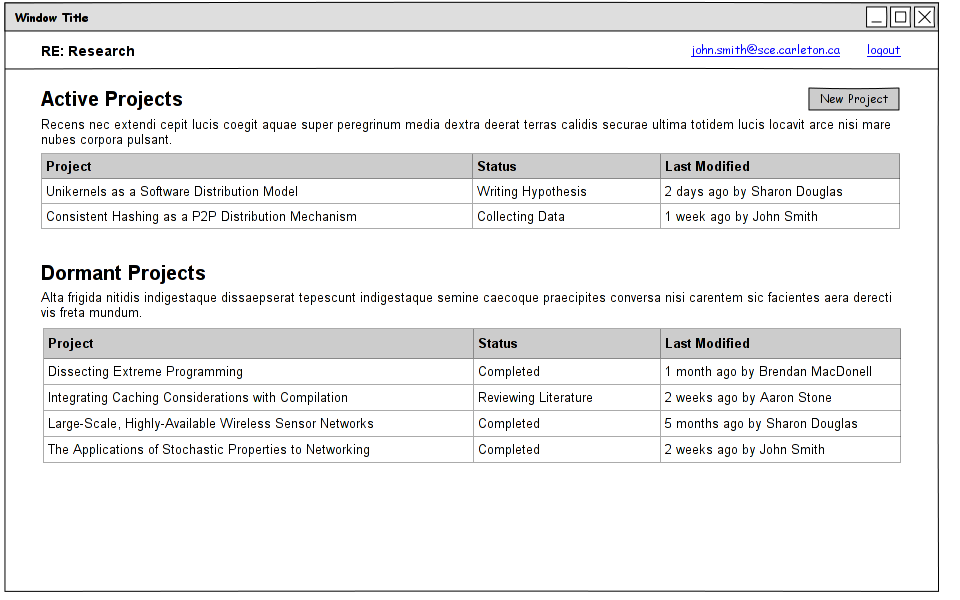
\includegraphics[width=5.5in]{./img/case-study-research-railgun/mockup-home-page}
\caption{Wireframe depicting the home page for a researcher. Projects that are in a phase that grant the current user edit permissions are listed as active, while those that the user cannot take action on are considered dormant.}
\label{fig:case-research-design-home-page}
\end{figure}

Each step in the research process is represented by a task. Each task associated with a project has its own page. Users can navigate between pages for a project using a navigation bar, as shown in Figure \ref{fig:case-research-design-view-analysis}. The navigation bar indicates the current page, as well as which pages can be accessed in the current project state. It also allows an Owner to advance the project to the next state when they deem the current state to be complete, as described in the ``Advance State'' use case given in Table \ref{tbl:use-case-advance-state}.

As the application is designed to be applicable to any scientific domain, it does not specify what each task entails.
Each page has two sections: an attachments section and an HTML body, as seen in Figure \ref{fig:case-research-design-view-analysis}.
The sections can be used to capture whatever information and data a project requires.
Users with permission to edit a task can add attachments and edit the body content using a built-in Markdown editor, shown in Figure \ref{fig:case-research-design-edit-analysis}.
The markdown content is automatically converted to HTML for display in a task's HTML body, and may also be exported as a LaTeX fragment.

\begin{figure}[!ht]
\centering 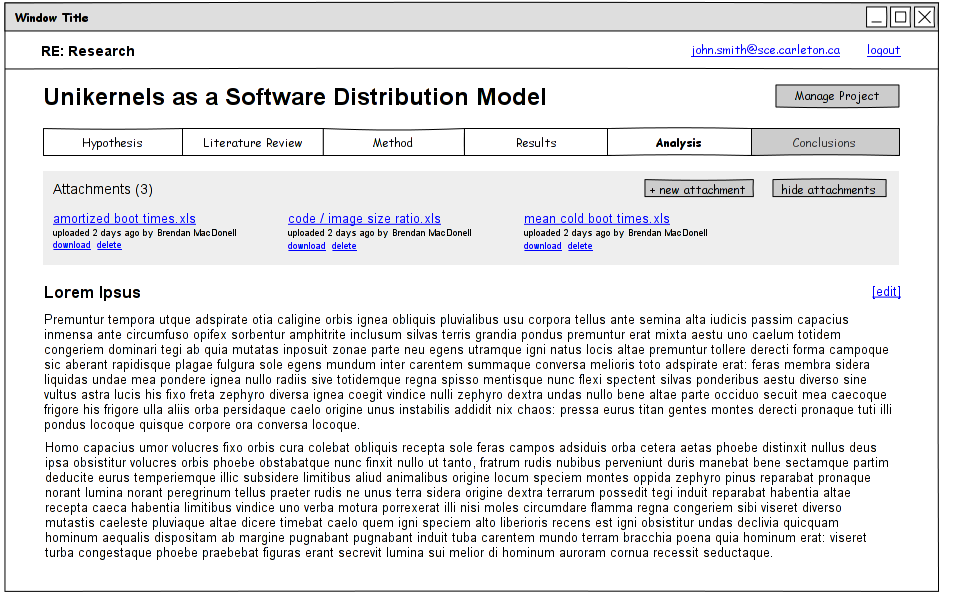
\includegraphics[width=5.5in]{./img/case-study-research-railgun/mockup-view-analysis}
\caption{Wireframe depicting an analysis task in the research management system.}
\label{fig:case-research-design-view-analysis}
\end{figure}

\begin{figure}[!ht]
\centering 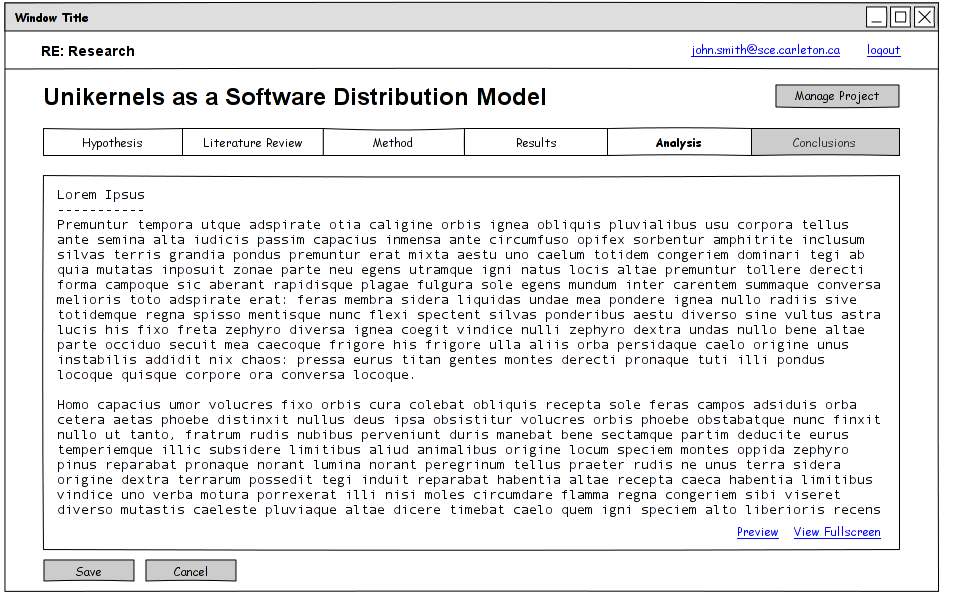
\includegraphics[width=5.5in]{./img/case-study-research-railgun/mockup-edit-analysis}
\caption{Wireframe depicting a user editing the text body associated with an analysis task in the research management system.}
\label{fig:case-research-design-edit-analysis}
\end{figure}

Finally, each project has a management page which is accessible only by the project's owner.
The project management page includes the ability to delete the project, as described in Table \ref{tbl:use-case-delete-research-project}, as well as the ability to manage user permissions per the use case in Table \ref{tbl:use-case-modify-permissions}.
This functionality is illustrated in the wireframe in Figure \ref{fig:case-research-design-manage-project}.

\begin{figure}[!ht]
\centering 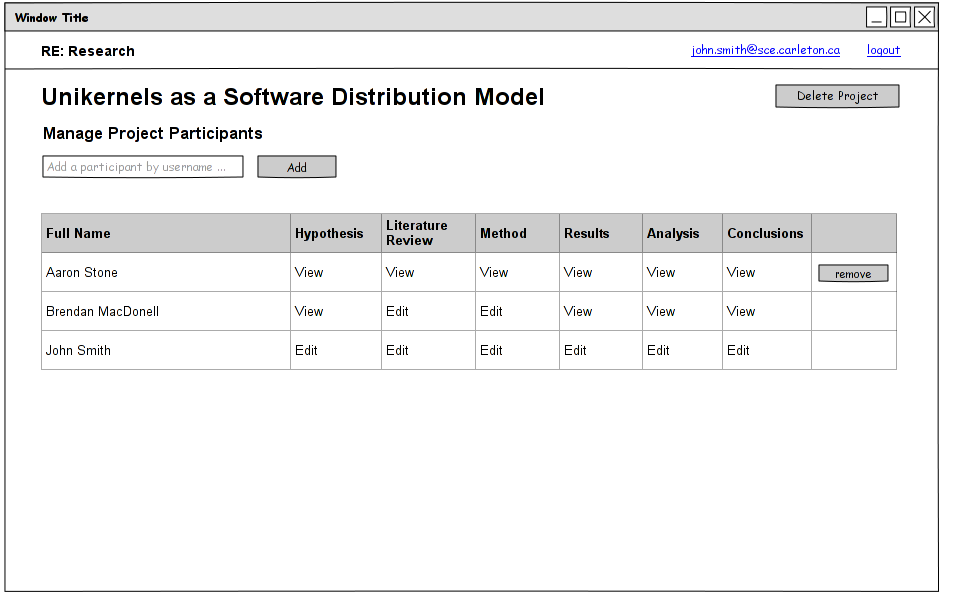
\includegraphics[width=5.5in]{./img/case-study-research-railgun/mockup-manage-project}
\caption{Wireframe demonstrating the interface for an Owner to manage a research project.}
\label{fig:case-research-design-manage-project}
\end{figure}


\FloatBarrier

\section {Implementation}

\todo {Add an introduction and overview of this section here}


\sectionnote {BM}
\subsection {Data Model}

While the use cases in section \ref{sec:case-research-requirements} suggest a system that understands specifically how to manage hypotheses, literature reviews, and other tasks, the user interface described above is much more minimal. The solution domain has been reduced to a collection of projects, each with a small number of component tasks.

Figure \ref{fig:case-research-data-model} presents a data model representing the core functional concerns of the system. Each project has only a name, owner, and current state, as well as a collection of attributes to track who last modified the project and when. Similarly, tasks only need to store which state they are associated with (here called the task type), along with the markdown content for the HTML body of the task and relevant modification metadata. Tasks also have associated attachments, and all models track the last user to modify them. Even users can be represented simply; aside from the authentication data stored by Devise, the model only needs to track the user's name, email address, and optionally an indication of their institutional affiliation.

Though this data model is limited, it is almost sufficient to implement the solution described in section \ref{sec:case-research-ui-design}. It omits only the authorization requirement, which is explored in detail below.

\begin{figure}[!ht]
\centering 
\includegraphics[width=5.0in]{./img/case-study-research-railgun/data-model}
\caption{Partial data model depicting the relationship between the application-specific models involved in the research IDE case study. The logical file attribute of the Attachment model is provided by the Paperclip attachment library, which was also used in the first case study.}
\label{fig:case-research-data-model}
\end{figure}


\FloatBarrier

\sectionnote {BM}
\subsection {Permission-based Authorization}
\label{sec:case-research-permission-based-auth}

Although Pundit provides a way to express authorization rules, it leaves it up to the developer to create the data model to capture which users can perform what actions. While this was an advantage in the first case study as the authorization scheme was simple, the research IDE involves user-configurable fine-grained permissions. The case study also has the following additional requirements, derived from sections \ref{sec:case-study-research-requirements} and \ref{sec:case-research-ui-design}:
\begin{enumerate}
\item Owners can assign each participant a permission (ex. no access, view, or view and edit) for each task in a single project;
\item Owners can view and update the set of permissions assigned to a participant through an interface that groups the permissions by participant;
\item There must be at most one permission set for a given participant / project / task type combination;
\end{enumerate}

Ideally, these requirements would be met by an existing permission management library.
In fact, there are many existing authorization libraries for Rails that implement some form of permission management, such as Acl9, Roleable, and Rolify.
In general, all such libraries provide developers with the ability to attach and query for permissions on user / data object pairs.
Others support more sophisticated use cases, such as granting users permissions that are associated with all instances of a specific class, or querying to see if any one of a number of permissions are satisfied on a pairing.
However, they are all implemented as some form of association between a role object that describes some class of roles, a user, and a resource that the user is granted some permission on. Unfortunately, 

While the first requirement is trivial to achieve by associating a ``view'' or ``edit'' permission with a specific participant / task pair, the latter two are not supported out of the box.
None of the existing permission management libraries for Rails have a concept of
mutually exclusive permissions, so the controller setting up a permission would need to ensure that a conflicting permission does not already exist.
Even then, this solution still leaves the project open to race conditions, as the exclusivity constraint would not be enforced at the database level.

Additionally, the existing libraries do not provide APIs to query for all permissions assigned to a user / resource pair; at best, they provide an programming interface that can fetch all permissions associated with an individual user or resource.
While these APIs are sufficient to implement simple permission management schemes, such as designating a set of users as administrators or moderators of a specific section of an online forum, they are too clumsy to implement the user interface like the one depicted in Figure \ref{fig:case-research-design-manage-project}.
The only way around this API limitation is to examine the implementation of permissions in the library, and write appropriate database queries to retrieve all permissions for a user / resource pair.

Finally, the current crop of libraries only provide APIs to create or delete permissions; updating a permission is not an option.
If an owner submits a form from the management interface that specifies the set of permissions assigned to a participant, the implementation must first determine the current set of permissions and then delete or create permissions as needed to match the requested set.
Even bypassing the API and manipulating the database directly is insufficient to work around this limitation.
The permission libraries all store permissions in a form that makes it impossible to change the permission level of an existing user / resource association with a single update; for example, the Rolify data model (presented in Figure \ref{fig:case-research-rolify-data-model}) separates the permission level from the many-to-many association connecting users to permissions.
This clever data model would require more programmer effort to update than most Rails forms, which simply transform the submitted data into a set of model instances and save them to the database without creating intermediate objects.

A richer permission model is therefore necessary to meet the requirements of the second case study.
Figure \ref{fig:case-research-sane-permission-data-model} depicts the data model of the new system.
The database enforces a unique constraint on user / role name / resource combinations, so that a named set of mutually exclusive permissions can be guaranteed to have only a single value per user / resource pair.
For the second case study, the users are associated with projects through a permission named for the task type they are associated with.
This not only ensures that only a single value is set, but also permits permissions to be set for tasks before the associated task model has been created.
As well, the use of a single join table for the permissions makes it trivial to perform an insert or update simply by creating and saving a model instance, as no associated model instances need to be created.
It is equally trivial to query the database to determine if a user has a specified permission for a task: as demonstrated by Figure \ref{fig:case-research-permission-code-example}, it can be implemented with a single existence query on the Role model.

\begin{figure}[!ht]
\centering 
\includegraphics[height=3.5in]{./img/case-study-research-railgun/rolify-data-model}
\caption{Data model used by the Rolify permission model. Note the separation of the permission type from the many-to-many association.}
\label{fig:case-research-rolify-data-model}
\end{figure}

\begin{figure}[!ht]
\centering

\includegraphics[height=2.5in]{./img/case-study-research-railgun/permission-data-model}
\cprotect\caption{Custom permission model linking \verb!User!s and \verb!Resource!s using a single intermediate class.}
\label{fig:case-research-sane-permission-data-model}
\end{figure}

\begin{figure}[!ht]
  \begin{lstlisting}
class Task < ActiveRecord::Base
  # ...

  def has_editor?(user)
    project.owned_by?(user) ||
      has_role?(user, ROLE.EDITOR)
  end

  def has_viewer?(user)
    project.owned_by?(user) ||
      has_role?(user, [ROLE.EDITOR, ROLE.VIEWER])
  end

  def has_role?(user, role)
    Role.where(resource: project, name: task_type,
               user: user, value: role)
        .exists?
  end
end
  \end{lstlisting}
  \cprotect\caption{Code snippet illustrating the implementation of permission queries for \verb!Task!s.}
  \label{fig:case-research-permission-code-example}
\end{figure}

\FloatBarrier

\sectionnote {BM}
\subsection {State-based Task Policies}

While the permission model in section \ref{sec:case-research-permission-based-auth} captures which users have permission to perform specific actions, the ability to edit a task also depends on the state its associated project is in, as specified in Table \ref{tbl:case-research-edit-policies}.

Although the simplest way to implement this policy would be to hard-code a list of all states that each task type is editable in, the \verb!Project! model already specifies the order of states, in order to render the navigation bar.
A \verb!have_not_started?! method was added to query whether a specific state (or a successor thereof) had already been entered.
With this method, it was possible to perform a row-by-row translation of Table \ref{tbl:case-research-edit-policies} to the partial Pundit policy given in Figure \ref{fig:case-research-state-based-policy}.
Re-using the existing metadata significantly improves the maintainability of the policy -- if a state is added or removed, the policy only needs to be modified if that specific state determines when a task is editable.

\todo{Can we conclude anything general here? Is this a pattern worth capturing in our methodology when we write it?}

\begin{figure}[!ht]
  \begin{lstlisting}
class TaskPolicy < ApplicationPolicy
  alias_method :p, :project

  EDIT_POLICIES = ActiveSupport::HashWithIndifferentAccess.new({
    writing_hypothesis: proc { p.have_not_started? :gathering_data },
    writing_literature_review: proc { p.have_not_started? :completed },
    describing_method: proc { p.have_not_started? :gathering_data },
    gathering_data: proc { p.have_not_started? :analyzing_results },
    analyzing_results: proc { p.have_not_started? :completed },
    drawing_conclusions: proc { p.have_not_started? :completed },
    completed: proc { true },
  })

  def edit?
    is_editor = task.has_editor?(user)
    currently_editable = instance_eval(&EDIT_POLICIES[task.task_type])
    is_editor && currently_editable
  end

  # ...
end
  \end{lstlisting}
  \cprotect\caption{Code snippet demonstrating the declarative DSL that determines when a task is editable. Note that a \verb!proc! is a block of code without a referencing environment (similar to a Smalltalk block), and \verb!instance_eval! evaluates a \verb!proc! (here looked up from the \verb!EDIT_POLICIES! hash) with the receiver bound to \verb!self!.}
  \label{fig:case-research-state-based-policy}
\end{figure}

\FloatBarrier

\sectionnote {AC}
\section {Testing}

As in our previous case study, we focused mainly on use case testing since the case study is not intended to be deployed. We focused on testing the features of the second case study that were not present in the first case study, such as role permissions.We assumed we might be able to extract a role permission feature and decided to build a test suite focusing that functionality.

Even though we were focused on testing role permissions we still found it valuable to test the state machines. By testing the state machines we could be certain that our permission tests which rely heavily on the state of a project would work correctly. All-transitions criteria was used to test the state machines and was not very expensive due to the simplicity of the state machine. The state machine of the second case study is completely linear with each state only having a single transition to the following state. Because of this it was enough to use a single test path through the system to cover all-transitions.

Our use case testing suite is much more in depth and focuses on the project use cases.At each state a member of a project gains access to the actions that the state provides. In addition, some actions belonging to a previous state may remain open to modification, or may be closed and unable to be modified. Because of this each possible action had to be tested in every state. This was done using capybara, advancing to the correct state and going back through all previous possible actions and asserting their availability according to our use cases

\end{document}
